

\chapter{Research Methodology}
\section{The dataset}
Before the model can be trained, tested and validated, I will need to acquire a dataset. The dataset of choice was the "Places365" dataset \cite{DBLP:journals/corr/ZhouKLTO16}. This dataset contains images of places, specifically streets, buildings, mountains, glaciers, and trees, but also contains images of objects and entities such as cars, planes, people and animals. Additionally, the set contains about 105,000 256x256 images across 65 classes split 60:20:20 for training, testing and validation respectively. The dataset is primarily used for image classification and analysis, but in my case, the task will be image colourisation \cite{landscape}.
\section{Data Preprocessing}
To ensure the models can interpret the data for training and testing, the data should be prepossessed. In my case, a \textbf{tensorflow pipeline} was used. The pipeline takes images in batches and will apply numerous transformations. These transformations may involve:  

\begin{enumerate}
  \item Decoding batches of images into numerical tensors is achieved using OpenCV's "imread" function.
  \item Creating input and targets. Inputs and outputs can be either grayscale input and RGB output for methods that perform RGB mapping, or \(L*\) and \(A*B\) respectively for methods that perform LAB mapping.
  \item Resizing the images to a constant size of 256 x 256 to ensure consistent dimensionality.
  \item Scaling each pixel of the image down to a range of [0,1]. This is done by dividing the colour channels from the images by the value of 255 (as RGB ranges between 0-255)
  \item Augmentation transformations are applied. These augmentations involve random cropping, flipping and zooming. Note that augmentation isn't used when using the testing set pipeline.
\end{enumerate}
\begin{figure}[H]
    \centering
    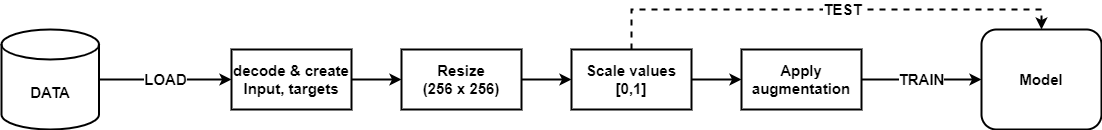
\includegraphics[width=1\columnwidth]{sections/figures/pipeline.png}
    \caption{Preprocessing pipeline}
    \label{fig:my_label}
\end{figure}






\pagebreak
\section{AutoEncoder method}
Here I've explored two AutoEncoder methods, Simple AutoEncoder and the Global AutoEncoder. 

Both models adopt the \(LAB\) colour space mapping since this colour space minimises the correlation between the three coordinate axes of the colour space.  




\subsection{Simple AutoEncoder}


\subsubsection*{Model Architecture}
\addcontentsline{toc}{subsubsection}{Model Architecture}
\begin{figure}[H]
    \centering
    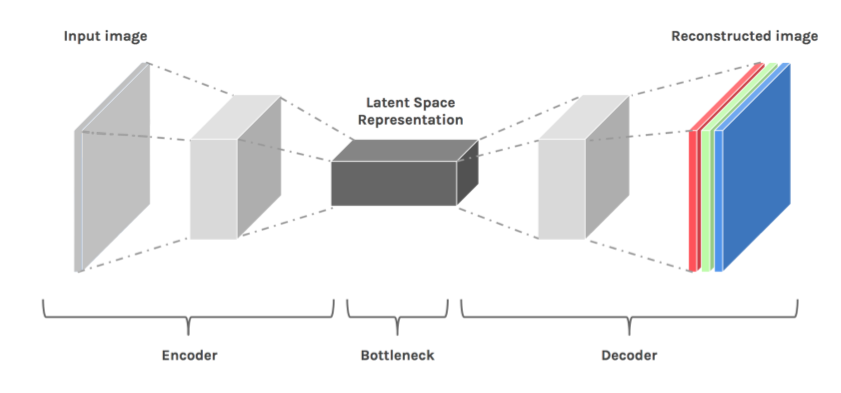
\includegraphics[width=0.7\columnwidth]{sections/figures/autoencoder.png}
    \caption{AutoEncoder architecture \cite{autoencoder2019}}
    \label{fig:my_label}
\end{figure}

The Simple AutoEncoder is regarded as the first method I experimented with during my research into image colourisation. The Architecture being used is based on \cite{IizukaSIGGRAPH2016} but without the Global Feature Extractor. For the sake of this report, this AutoEncoder will be referred to as \textbf{Simple AutoEncoder}.

This architecture is considered simple as out of all the methods I have experimented with, this model uses the fewest amount of parameters.

The basic anatomy of this AutoEncoder involves three distinct parts: the Encoder unit, Bottleneck \& the Decoder unit.

\subsubsection*{Encoder unit}
\addcontentsline{toc}{subsubsection}{Encoder unit}

The low-level features are encapsulated as part of the encoder. The encoder extracts features from the input image and comprises 10 convolution layers, each consisting of 3x3 kernels. The input of the encoder is the grayscale image, which represents H x W x 1, where H and W refer to the image's height and width. The result of the encoder represents H/8 x W/8 x 512. Setting each layer's padding to "same" helps to preserve the original image size. Strides are used at each convolution layer, this helps to reduce the output of the image by 50\%. Ultimately, the output image is decomposed into a latent space representation.

\subsubsection*{Bottleneck unit}
\addcontentsline{toc}{subsubsection}{Bottleneck unit}
The bottleneck unit of the autoencoder is the unit in the middle of the network that has the smallest number of neurons. This unit provides the lowest level of abstraction for the input data and forces the autoencoder to learn to compress the input data into a lower-dimensional representation.

\subsubsection*{Decoder unit}
\addcontentsline{toc}{subsubsection}{Decoder unit}


The decoder takes the bottleneck output as input and uses it to estimate the colours of the image. During this process, several upsample layers are used to increase the spatial H x W of the feature maps, using the UpSample2D. The produced output is the roughly estimated A*B* channels, with the H x W x 2 volume representation. The output of the decoder is then concatenated with the input grayscale channel to form the full L*A*B* image, which is then converted to RGB representation.
\pagebreak
\subsection{Global AutoEncoder method}

\subsubsection*{Model Architecture}
\addcontentsline{toc}{subsubsection}{Model Architecture}

\begin{figure}[H]
    \centering
    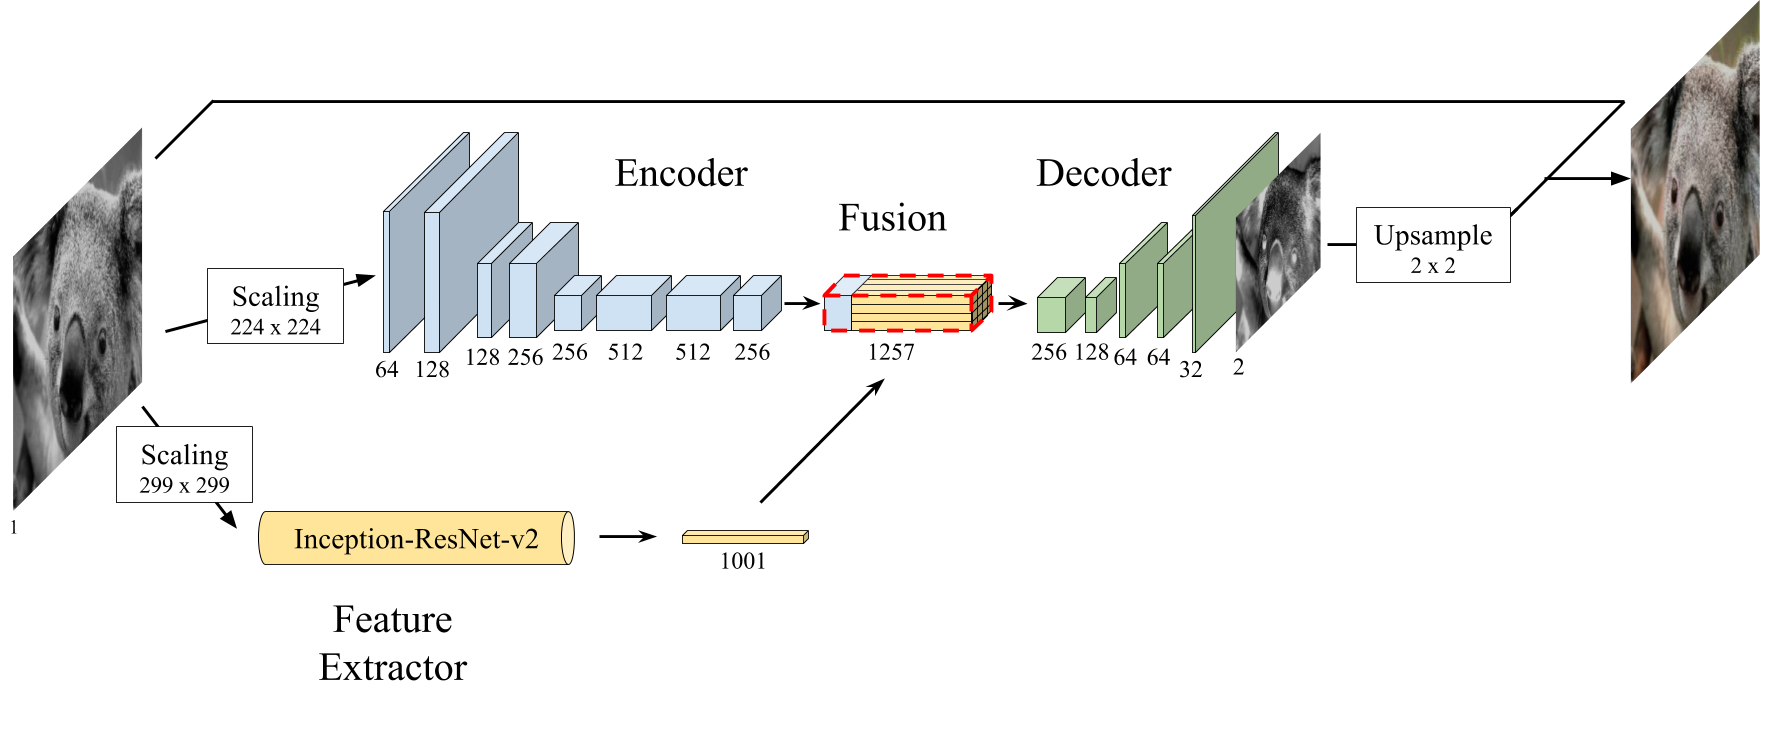
\includegraphics[width=1\columnwidth]{sections/figures/model.png}
    \caption{Deep Koalarization  architecture}
    \label{fig:my_label}
\end{figure}

The base architecture used for the image colourisation model is a form of an autoencoder and was developed by Federico Baldassarre, Diego Gonzalez-Morin and Lucas Rodes-Guirao \cite{deepkoal2017}. Their model was based on the authors of \cite{IizukaSIGGRAPH2016} (as seen in Figure 11).

\begin{figure}[H]
    \centering
    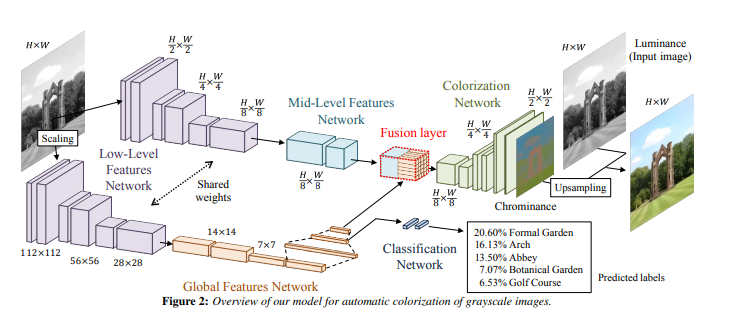
\includegraphics[width=0.8\columnwidth]{sections/figures/different_model.PNG}
    \caption{Let there be color architecture}
    \label{fig:my_label}
\end{figure}

\cite{deepkoal2017} (figure 3.3) use a pre-trained model (Inception-Resnet-V2) as a global feature extractor, whereas \cite{IizukaSIGGRAPH2016} (figure 3.4) use their own trained model for this purpose. The use of a pre-trained model for the global feature extractor eliminates the need to train a separate model, as the inception-ResNet-v2 has been trained over 1000 classes of images.

This model consists of four parts: the encoder, global feature extractor, fusion layer, and decoder. The encoder takes in the L channel (grayscale) and extracts low-level features. The input is also fed into a global feature extractor (GFE) which extracts global features. The fusion layer then combines the outputs of GFE and encoder. The fusion layer's output is then fed into the decoder, which does the colourisation task by mapping outputs to their corresponding colour channels.
 
The base AutoEncoder (without the global feature extractor) architecture used is identical to the previous simple AutoEncoder mentioned previous section, hence I will not go over the implementation again for this method, but rather will go over the highlighted differences. For the sake of this report, I will be referring to this architecture as \textbf{Global AutoEncoder}.

\subsubsection*{Global feature extractor}
\addcontentsline{toc}{subsubsection}{Global feature extractor}


The global feature extractor helps to identify and extract global features from the image and outputs a class distribution. The model is a pre-trained inception-resnet. It takes as input a grayscale image input which is upscaled to H x W of 299 x 299 respectively. The output of GFE will result in the image representing a 1000-dimensional class distribution vector. The point of the GFE is to indicate the class of the image from the given input so that it can help identify relevant colours. For instance, if the GFE identified the image as being an indoor room consisting of furniture, the GFE will mitigate the encoder from being biased, so that it will add appropriate colours for furniture, rather than sky or grass colours. 

\subsubsection*{Fusion Layer}
\addcontentsline{toc}{subsubsection}{Fusion Layer}



The fusion layer combines the output of the GFE (a 256 dimensional vector) and the encoder. The use of the fusion layer results with a H/8 x W/8 x 256 layer. This effectively merges the information gathered from the GFE and the encoder into one layer. The formula for fusion can be seen as:
\begin{equation}
y_{u,v}^{fusion} = \sigma \left ( b + W \begin{bmatrix}y^{global} \\y_{u,v}^{mid}  \end{bmatrix} \right )
\end{equation}

Where \(y_{u,v}^{fusion}\) is the fusion of features \(u,v\). Where \(y^{global} \) is the global feature vector and \(y_{u,v}^{mid} \) is the mid level feature at (\(u,v\)). \(W\) is the weights and \(B\) is the bias. Both, \(W\) and \(B\) are trainable variables. 


\pagebreak
\section{Conditional GAN method}
I have experimented with two different types of conditional GANs, ChromaGAN and Pix2Pix, to see if they perform better than the AutoEncoder methods that were discussed earlier.

\subsection{Pix2Pix GAN}
\begin{figure}[H]
    \centering
    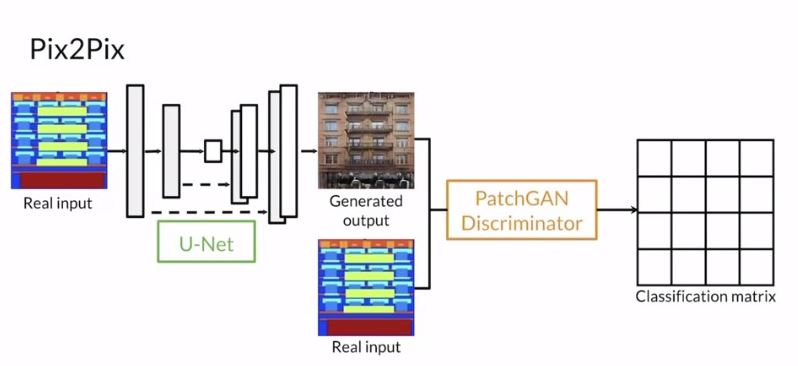
\includegraphics[width=1\columnwidth]{sections/figures/pix2pix_architecture.JPG}
    \caption{Pix2Pix Architecture \cite{DBLP:journals/corr/IsolaZZE16}}
    \label{fig:my_label}
\end{figure}

Pix2Pix is a category of cGAN and is used for image to image translation. This network not only can learn the mapping from an input image to an output image but also learns the loss function to train this mapping.

Pix2pix was developed as a more sophisticated approach to image-to-image translation, compared to the basic CNN method which simply minimizes the Euclidean distance between the predicted and ground truth pixels. However, it was seen that this method would result in a blurry output, as the Euclidean distance is minimized by averaging up all the outputs, causing the blurring effect.

In brief, the architecture works by learning a loss function that tries to classify the output image as being either real or fake, while simultaneously training a generative model to minimise this loss. Blurry images will not be tolerated as they will easily look fake.

\subsubsection*{U-NET Architecture (Generator)}
\addcontentsline{toc}{subsubsection}{U-NET Architecture (Generator)}

\begin{figure}[H]
    \centering
    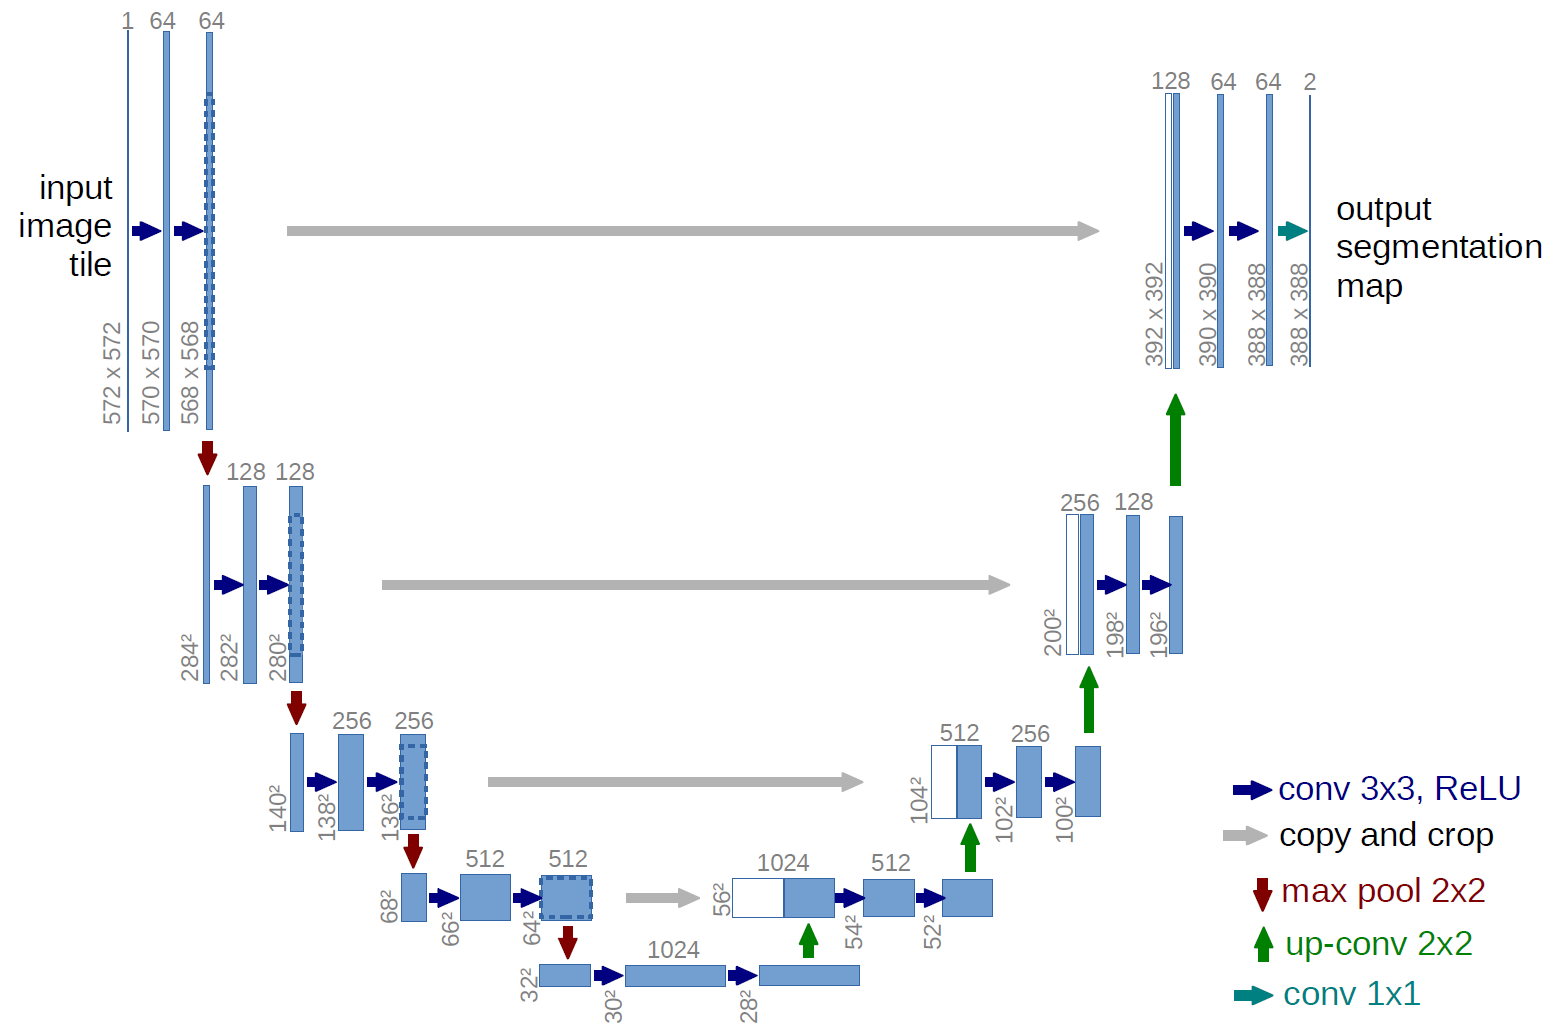
\includegraphics[width=0.7\columnwidth]{sections/figures/U-net.JPG}
    \caption{U-NET model \cite{RFB15a}}
    \label{fig:my_label}
\end{figure}

The most important aspect of the cGAN is the generator, as this is responsible for generating the coloured output. As discussed earlier, Pix2Pix can only work if the output image is not blurry, and having such blurry images will only help the discriminator in identifying the generated images. The AutoEncoder method I discussed earlier uses an encoder-decoder network. In these networks, the input image is progressively decomposed through the layers until it reaches a bottleneck, and from there the process is reversed. However, since the information is constantly being decomposed, information that helped retain the structures of the input image is risked being lost.

To mitigate this issue, the generator can utilise skip connections which creates the shape of a "U-Net". This architecture adds skip connections between each \(ith\) and the \(n - i\), where \(n\) represents the number of layers in the network. Using skip connection help pass information between the encoder and the decoder, information that involves the underlining structure, which helps mitigate the blurry effect, and also why this architecture can use the RGB mapping, previously sought to produce blurry images an AutoEncoder. 

\subsubsection*{PatchGan Architecture (Discriminator)}
\addcontentsline{toc}{subsubsection}{PatchGan Architecture (Discriminator)}
\begin{figure}[H]
    \centering
    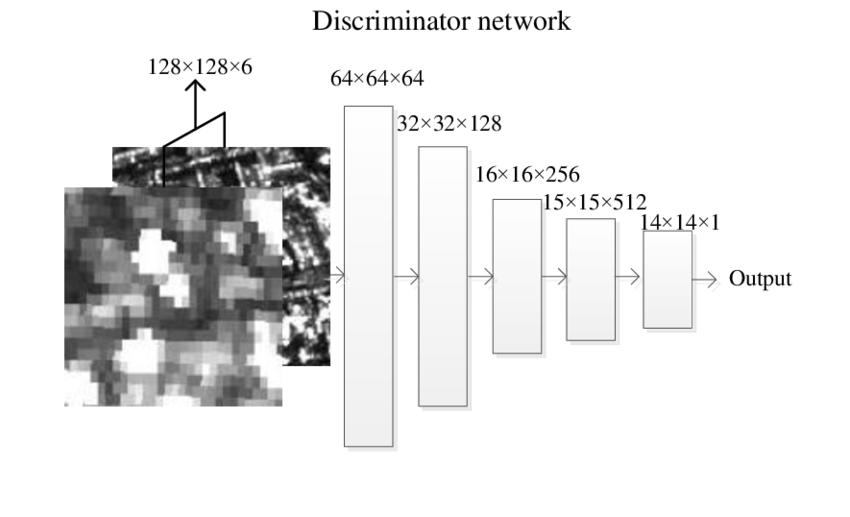
\includegraphics[width=0.7\columnwidth]{sections/figures/PatchGAN.png}
    \caption{PatchGAN model \cite{ao_2018}}
    \label{fig:my_label}
\end{figure}
The architecture of the discriminator used in Pix2Pix is based on the Markovian discriminator architecture, also known as patchGAN \cite{etal_2018}. PatchGAN is used for binary classification. This discriminator is used to address blurry images when using L1 loss and L2 loss on high frequency, however, it turned out that having L1 loss switched to low frequency helped mitigate this issue. The way this architecture works is by dividing the input image into \(N x N\) patches and then identifying each patch of the image as either real or fake. 

The size of the \(N\) patch was noted to influence the output of the image. Using smaller patches was reported to speed up training time, and the results often looked high quality. 
The discriminator is created using convolutional layers and LeakyRelU was used as this was reported to help solve the vanishing gradient problem \cite{brownlee_2020}. 





\newpage
\subsection{ChromaGAN}

\begin{figure}[H]
    \centering
    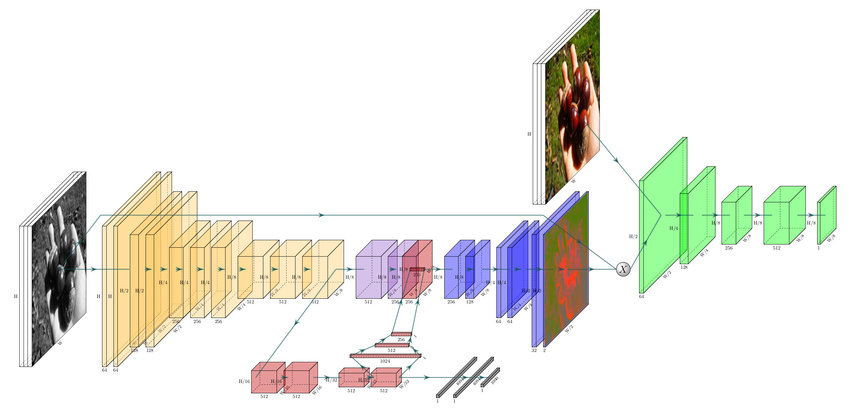
\includegraphics[width=1\columnwidth]{sections/figures/ChromaGAN_architecture.png}
    \caption{ChromaGAN Architecture}
    \label{fig:my_label}
\end{figure}

The ChromaGAN architecture is a conditional GAN. This architecture was developed by researchers from the University Pompeu Fabra \cite{DBLP:journals/corr/abs-1907-09837}. This architecture was developed for the purpose of colourisation of grayscale images. 

The difference between this architecture and the Pix2Pix method is the generator. ChromaGAN uses an AutoEncoder, which is similar to the global AutoEncoder discussed earlier. It performs LAB mapping and utilises a pre-trained global feature extractor, which is used to learn the class distribution vector. The distribution vector enables the information about the probability distribution within the semantic information contained within input \(L\), and this helps improve the colourisation performance without the need for a labelled dataset.




\subsubsection*{Generator Architecture}
\addcontentsline{toc}{subsubsection}{Generator Architecture}

The generator of the ChromaGAN is a network divided into two subnetworks: the AutoEncoder (yellow, purple and blue parts shown in figure 3.7) and the global feature extractor (red parts shown in figure 3.7). Here, I will be denoting both networks as \(G^1\) and  \(G^2\). Both \(G^1\) and \(G^2\) take as input a \(H x W\) image. \(G^1\) outputs chrominance information represented as \((a,b) = G^1(L)\), and \(G^2\) outputs the class distribution vector \(y = G^2(L)\). \(G^2\) can only take in the input of channel size of 3, so the input image requires broadcasting, which involves concatenating the input image three times \([L,L,L]\). \(G^2\) uses the pre-trained VGG-16 weights, but they are kept unfrozen during the process of training.

The encoder output of \(G^1\) (represented in orange in figure 3.7) is then fused with the class distribution output produced from \(G^2\). The fused output is then fed as input into the last stage of \(G^1\), which is the decoder. The decoder will process this information through six modules of CNN layers with ReLu activation functions, along with two upsampling layers between them. The produced output is then concatenated with the input to form the full coloured image which will then be used against the adversary.

\subsubsection*{Discriminator Architecture}
\addcontentsline{toc}{subsubsection}{Discriminator Architecture}

The discriminator of the ChromoGAN is the patchGAN. The patchGAN discriminator has already been discussed as pix2pix also uses the same discriminator. To be brief, it is noted that this architecture exceeds when working when capturing low-frequency structure of the input image, however, fails when working at high frequency. This process involves dividing the \(H x W\) input into patches and then classifies each individual patch of the image. The size of the patch was noted to influence the performance, as using smaller patches helped speed up performance and increase the quality of the input image produced by the generator.




\pagebreak
\section{Training and evaluation}
 Out of the \textbf{105,000} samples from the Places dataset, \textbf{84,000} was reserved for training whilst \textbf{21,000} was used for\textbf{ testing and evaluation}.

All models were trained using \textbf{Slurm Facility} which is an workload manager for scheduling jobs for large scale cluster. \cite{enwiki:1078654743}. The university provided me this service, and it allowed me to train the models practically for free.

Unfortunately, I could not leverage the time I had for optimisation. As a compromise, I will be sticking to the author's chosen hyper-parameter and will be performing quantitative testing using evaluation metrics. In the interim, I have performed tuning using a smaller dataset, please refer to Appendix B for this. 

\textbf{Nvidia Cuda} Toolkit with\textbf{ Nvidia Tesla M10} were used to enable GPU acceleration for faster training. The training time between each method was different, as some methods took 1 day to train whereas others took up to 4 days. 


\subsection{Objective functions}
The objective function is a key component in deep learning because it provides a way to find the optimal solution \cite{kronovet_2017}. The objectives may involve minimising or maximising a value. This value may represent an error used to quantify the distance between the predictions and the targets. The algorithm will continuously configure the model's parameters to minimise this error. Therefore, the use of an objective is essential in deep learning.

Since I have researched the 4 methods discussed throughout this section, it's known that each method has its own unique objective function.

\subsubsection*{AutoEncoder Objective function}
\addcontentsline{toc}{subsubsection}{AutoEncoder Objective function}
Both AutoEncoder methods discussed so far use the same objective function. This objective function can be defined as computing the distance between the estimated output and the target output. A Mean Square Error loss function is used to quantify the error between the estimated pixel and the target pixel. The objective function can be denoted as the following formula:
\begin{equation}
C(X,\theta ) = \frac{1}{2HW}\sum_{k \in (a,b)}^{}\sum_{i=1}^{H}\sum_{j=1}^{W}||X_{k_{i,j}} - \hat{X}_{k_{i,j}} ||^2
\end{equation}
Where \(\theta\) represents the parameters of the model, \( X_{k_{i,j}} \) and \( \hat{X}_{k_{i,j}} \) denote the \(i,jth\) pixel value of the \(kth\) channel value contained in the target and reconstructed predicted image respectively. The \(||.||^2\) is the euclidean distance used to compute the difference between \( X_{k_{i,j}} \) and \( \hat{X}_{k_{i,j}} \). 
% 
Both methods employ the same optimiser which is Adam to minimise this objective. This optimiser is preferred because it can handle sparse gradients on noisy problems such as natural language and computer vision \cite{brownlee_2021}. 
Both methods have an initial learning rate set at 0.0001.



\subsubsection*{Pix2Pix Objective function}
\addcontentsline{toc}{subsubsection}{Pix2Pix Objective function}
The objective function for Pix2Pix is unique compared to the AutoEncoder methods mentioned above, as both entities of the cGAN, the generator and the discriminator are competing against one another over the same objective. The anatomy of how Pix2Pix performs is through an objective function expressed below:
$$
\begin{aligned}
\arg \min _{G} \max _{D} \mathcal{L}_{c G A N}(G, D)+\lambda \mathcal{L}_{L 1}(G)
\end{aligned}
$$
Where \(G\) represents the Generator that is tasked to minimise the objective against the discriminator \(D\) which tries to maximise it. In addition to the objective, a \(\mathcal{L}_{L 1}(G)\) cost is added, and can be expressed as:

$$
\mathcal{L}_{L 1}(G)=\mathbb{E}_{x, y, z}\left[\|y-G(x, z)\|_{1}\right]
$$
The \(L1\) distance is used instead of the \(L2\) as it was discussed earlier that using \(L1\) encouraged less blurring in images.

The Adam optimiser is used to minimise this objective with the learning rate set at \(2e-4\) and the momentum parameters set at \(\beta_1 = 0.5\) and \(\beta_2 = 0.999\).



\subsubsection*{ChromaGAN Objective function}
\addcontentsline{toc}{subsubsection}{ChromaGAN Objective function}
The objective of the ChromaGAN is similar to Pix2Pix, both generator and discriminator are continuously competing against one another. The objective is defined by the following formula:
\begin{equation}
\arg \min _{G} \max _{D} \mathcal{L}_{c G A N}(G, D)
\end{equation}
However, the difference lies within the \(\mathcal{L}_{c G A N}(G, D)\) objective function:
\begin{equation}
\mathcal{L}_{c G A N}(G, D)=\mathcal{L}_{\mathrm{e}}\left(\mathcal{G}_{\theta_{1}}^{1}\right)+\lambda_{\mathrm{g}} \mathcal{L}_{\mathrm{g}}\left(\mathcal{G}_{\theta_{1}}^{1}, D_{w}\right)+\lambda_{\mathrm{s}} \mathcal{L}_{\mathrm{s}}\left(\mathcal{G}_{\theta_{2}}^{2}\right)
\end{equation}

The first term in the equation, $\mathcal{L}_{\mathrm{e}}\left(\mathcal{G}_{\theta_{1}}^{1}\right)$, is the color error loss of the encoder-decoder part of the generator. The second term, $\lambda_{\mathrm{s}} \mathcal{L}_{\mathrm{s}}\left(\mathcal{G}_{\theta_{2}}^{2}\right)$, is the class distribution loss produced by the VGG-16 model.

This objective is minimised using the Adam optimiser which has a set learning rate of 2e-5 and has the momentum parameters set at \(\beta_1 = 0.5\) and \(\beta_2 = 0.999\).


\pagebreak
\subsection{Evaluation Metrics}
% Due to the black box nature of the Deep Learning models, deploying them requires extensive verification and testing to gain insights into the decision-making process \cite{electronics10050593}. Without this, determining the success of the model's performance on unseen data, and identifying whether the algorithms have overfitted the training data will be difficult. Hence, the need for evaluation metrics is essential to help verify the model's performance on unseen data. This is also known as generalisation; the goal of every deep learning model is to have good generalisation \cite{enwiki:1073306062}.

% However, finding a quantitative metric to evaluate the performance of all discussed methods is a challenging task, as not all methods could rely on an agreed method of evaluation. Fortunately, the authors of the methods all used common methods: PSNR, SSIM and Perception test.
Due to the black box nature of Deep Learning models, extensive testing and validation is require to gain insight into the decision-making process \cite{electronics10050593}. This can be done using various techniques. Here, I will be using PSNR, SSIM and Naturalness study to conduct me evaluation.

\subsubsection*{PSNR score}
\addcontentsline{toc}{subsubsection}{PSNR score}
The Peak Signal-to-Noise Ratio (PSNR) is an objective metrics used to calculate the ratio in decibels between two images. This ratio is used to measure the quality between the target image and the original image. The ratio is used to indicate the quality of the output image; the higher the ratio, the better the quality of the output image. It's essentially another way of estimating the similarities between the colourised image and the ground truth \cite{Chauhan2018}. The formula for calculating the PSNR score is as follows:
\begin{equation}
\begin{gathered}
P S N R=10 \log _{10}\left(\frac{M A X_{l}^{2}}{M S E}\right) \\
M S E=\frac{1}{m n} \sum_{i=0}^{m-1} \sum_{j=0}^{n-1}[I(i, j)-K(i, j)]^{2} 
\end{gathered}
\cite{anon_2014}
\end{equation}
Where \(M A X_{l}\) represents the maximum pixel value of the image, whereas the \(M S E\) is used to measure the difference between the original and target image.


\subsubsection*{SSIM score}
\addcontentsline{toc}{subsubsection}{SSIM score}
SSIM (structural similarity index measure) is another objective metric used for quantifying the differences or similarity between two images. This metric is meant to serve as an alternative to the PSNR score, and unlike the PSNR score, the SSIM score can capture visible structure of the image \cite{1284395}.

The SSIM index is calculated as:
\begin{equation}
\operatorname{SSIM}(f, g)=l(f, g) c(f, g) s(f, g)
\end{equation}
where
\begin{equation}
\left\{\begin{array}{l}
l(f, g)=\frac{2 \mu_{f} \mu_{g}+C_{1}}{\mu_{f}^{2}+\mu_{g}^{2}+C_{1}} \\
c(f, g)=\frac{2 \sigma_{f} \sigma_{g}+C_{2}}{\sigma_{f}^{2}+\sigma_{g}^{2}+C_{2}} \\
s(f, g)=\frac{\sigma_{f g}+C_{3}}{\sigma_{f} \sigma_{g}+C_{3}}
\end{array}\right.
\cite{5596999}
\end{equation}

The first term is the luminance comparison of the two images. The second term is the contrast comparison and the last term is used for structural comparison of the two images. A SSIM of 1 means both images are the same, whereas a high SSIM denotes a high similarity and a low SSIM means there's little to nothing in common between the two images. 



\pagebreak
\subsubsection*{Naturalness study}
\addcontentsline{toc}{subsubsection}{Naturalness study}
The naturalness study is another form of quantitative evaluation, however, unlike previous objective metrics (PSNR & SSIM), this method relies on human opinion. The way the natural study works is by providing a naturalness perception test to volunteers. Each volunteer was given instructions (see figure 3.8 below) and their job is to agree or disagree on whether the colours of the image looked natural or not.

\begin{figure}[H]
    \centering
    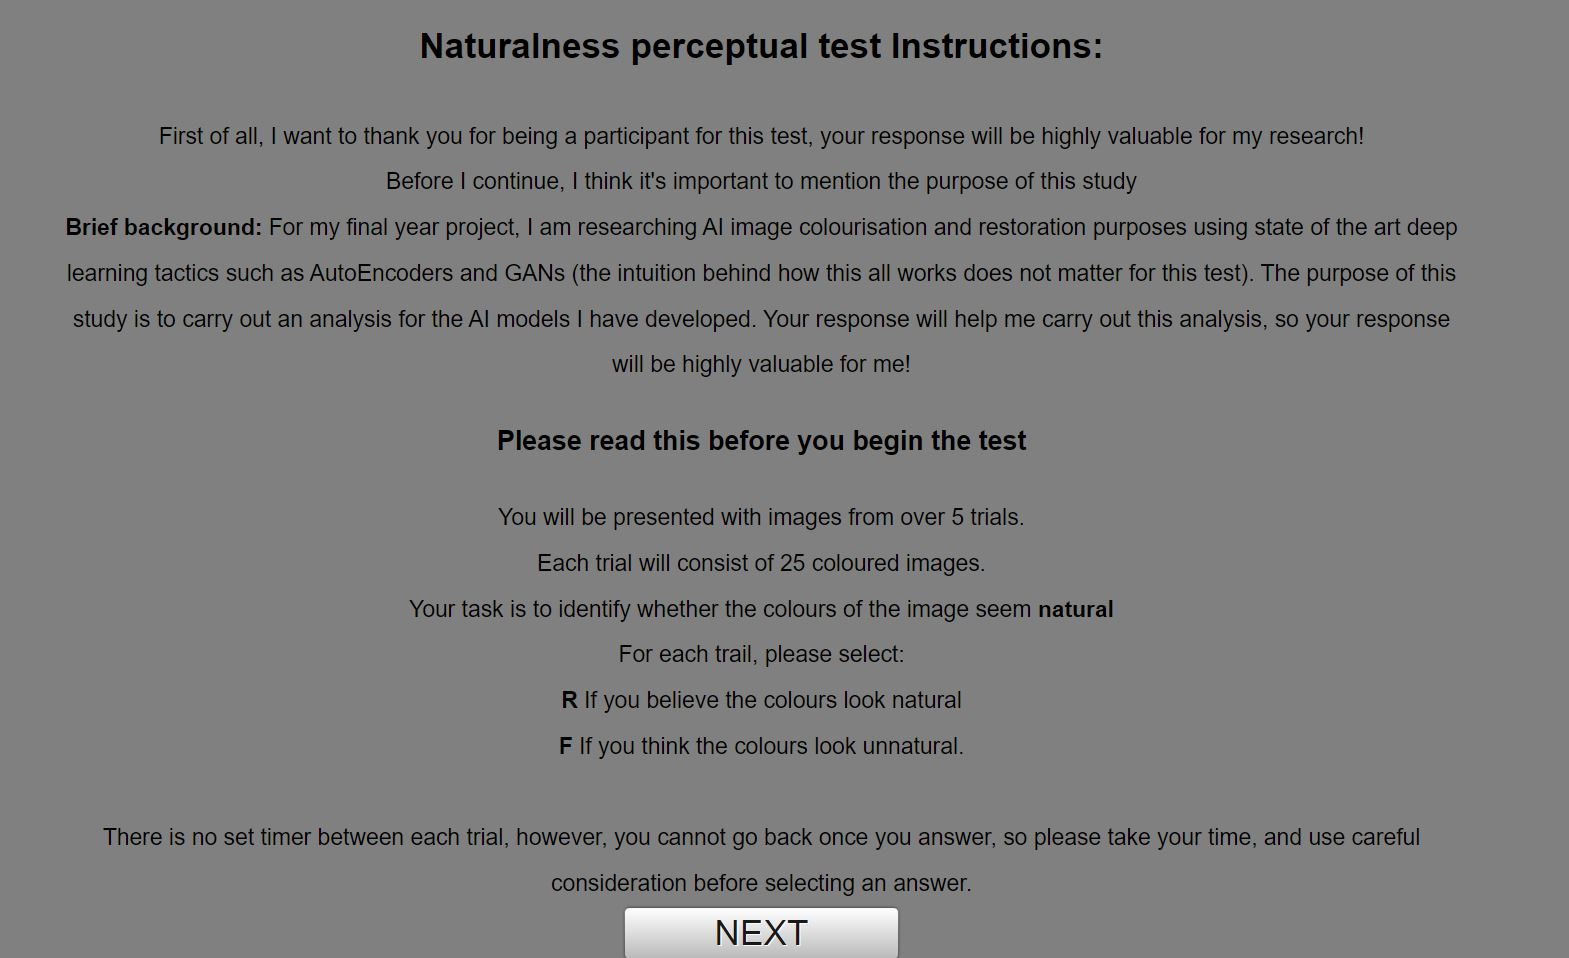
\includegraphics[width=0.8\columnwidth]{sections/figures/naturalness_study_instructions.JPG}
    \caption{Naturalness Perceptual test instructions}
    \label{fig:my_label}
\end{figure}



For example, figure 3.9 is one of the many images presented to the user, they needed to press R or F to answer.

\begin{figure}[H]
     \centering
     \begin{subfigure}[b]{0.3\textwidth}
         \centering
         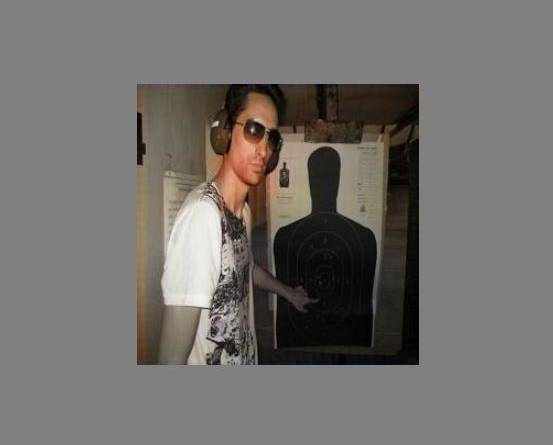
\includegraphics[width=\textwidth]{sections/figures/study_1.JPG}
         \caption{}
         \label{fig:y equals x}
     \end{subfigure}
     \hfill
     \begin{subfigure}[b]{0.3\textwidth}
         \centering
         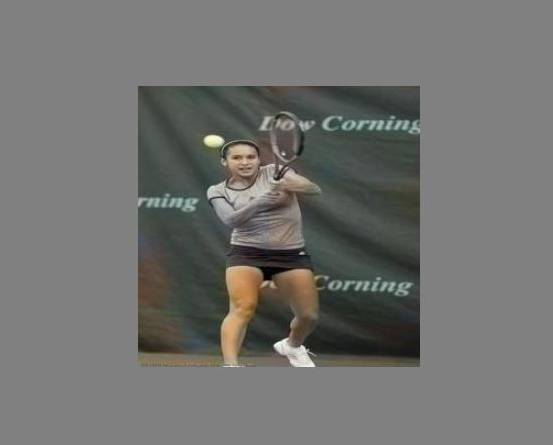
\includegraphics[width=\textwidth]{sections/figures/study_2.JPG}
         \caption{}
         \label{fig:three sin x}
     \end{subfigure}
     \hfill
     \begin{subfigure}[b]{0.3\textwidth}
         \centering
         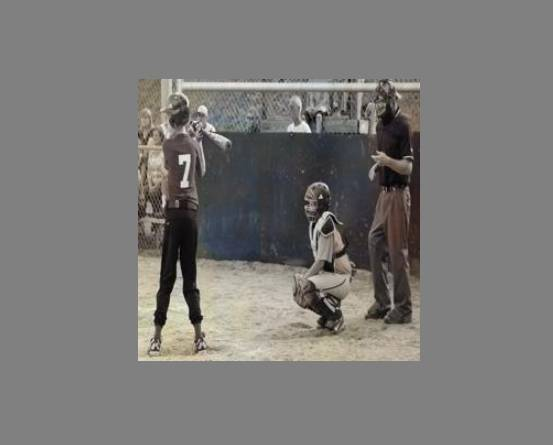
\includegraphics[width=\textwidth]{sections/figures/study_3.JPG}
         \caption{}
         \label{fig:five over x}
     \end{subfigure}
        \caption{Three simple graphs}
        \label{fig:three graphs}
\end{figure}



The study was carried out using a website called \(testable.org\) which is primarily used for experimenting with people's behaviour and perception using surveys and tests. 

This technique was used as calculating accuracy turned out to be unreliable because the calculated accuracy is used to calculate the similarities between two images and does not takes into consideration the naturalness. This could only be achieved by carrying out a study, hence the purpose of this method.











%REFERENCE 1 : https://machinelearningmastery.com/adam-optimization-algorithm-for-deep-learning/#:~:text=Adam%20is%20a%20replacement%20optimization,sparse%20gradients%20on%20noisy%20problems.

%REFERENCE 2: http://kronosapiens.github.io/blog/2017/03/28/objective-functions-in-machine-learning.html

%REFERENCE 3: chrome-extension://cbnaodkpfinfiipjblikofhlhlcickei/src/pdfviewer/web/viewer.html?file=file:///C:/Users/munee/Downloads/electronics-10-00593-v3.pdf

%REFERENCE 4: https://vitalflux.com/hold-out-method-for-training-machine-learning-model/

%REFERENCE 5: https://www.sciencedirect.com/topics/engineering/peak-signal#:~:text=PSNR%20is%20defined%20as%20the,noise%20that%20affects%20representation%20fidelity.

%REFERENCE 6:https://www.matlabclass.com/2014/02/how-to-calculate-psnr-peak-signal-to.html

%REFERENCE 7: https://slurm.schedmd.com/overview.html


